\id{МРНТИ 65.33.03}{}

\begin{articleheader}
\sectionwithauthors{А.И. Кабылда, А.С. Жармаханова, Ж.С. Кожухова}{СРАВНЕНИЕ КАЧЕСТВЕННЫХ характеристик ПЛОДОВО-ЯГОДНЫХ ПОРОШКОВ ДЛЯ ВИТАМИНИЗованных ЭКСТРУДИРОВАННЫХ БЕЗГЛЮТЕНОВЫХ СНЭКОВ}

{\bfseries А.И. Кабылда\authorid,
А.С. Жармаханова\authorid,
Ж.С. Кожухова\textsuperscript{\envelope } \authorid}
\end{articleheader}

\begin{affiliation}
\emph{АФ ТОО «Казахский научный исследовательский институт перерабатывающей и пищевой промышленности», Астана, Казахстан,}

\raggedright \textsuperscript{\envelope }{\em Автор-корреспондент: \href{mailto:jansa1612@gmail.com}{\nolinkurl{jansa1612@gmail.com}}}
\end{affiliation}

Настоящий обзор направлен на сравнение качественных характеристик
плодово-ягодных порошков в разработке витаминизованных безглютеновых
снэков, что представляет собой важную задачу в области функционального
питания. В статье рассматриваются порошки различных плодово-ягодных
культур, а именно банан, яблоко, клюква, черная смородина, черника,
облепиха, шиповник. Эти виды сырья исследуются с точки зрения их
физико-химических показателей и витаминной ценности, а именно
рассматривается содержание белка, жира, углеводов, клетчатки, витаминов
B1, A, C, PP.

На основе проведенного сравнения было определено, какие плодово-ягодные
порошки обладают наибольшими уровнями витаминов и питательных веществ,
что позволяет улучшить питательную ценность конечных продуктов.
Полученные результаты подтверждают возможность использования
плодово-ягодных порошков для создания витаминизированных безглютеновых
снеков с улучшенными функциональными и вкусовыми свойствами.

Работа направлена на расширение ассортимента безглютеновых продуктов,
что особенно актуально в условиях роста интереса к здоровому питанию и
потребности в функциональных продуктах питания. Создание таких снэков с
улучшенными органолептическими и питательными характеристиками будет
способствовать улучшению рациона питания людей с глютеновой
непереносимостью, а также всех, кто стремится к здоровому образу жизни.
Это подтверждает возможность использования плодово-ягодных порошков для
создания витаминизированных безглютеновых снеков с улучшенными
функциональными свойствами.

{\bfseries Ключевые слова:} переработка, технология, сырье, безглютеновая
продукция, безглютеновые экструдированные снэки, плодово-ягодные
порошки, витаминный состав, физико-химические показатели.

\begin{articleheader}
{\bfseries ЖЕМІС-ЖИДЕК ҰНТАҒЫНЫҢ ВИТАМИНДЕНДІРІЛГЕН ЭКСТРУЗИЯЛАНҒАН ГЛЮТЕНСІЗ СНЕКТЕР ҮШІН САПАЛЫҚ СИПАТТАМАЛАРЫН САЛЫСТЫРУ}

{\bfseries
А.И. Қабылда,
А.С. Жармаханова,
Ж.С. Кожухова\textsuperscript{\envelope }}
\end{articleheader}

\begin{affiliation}
\emph{Астана филиалы ЖШС «Қазақ қайта өңдеу және тағам өнеркәсіптері ғылыми-зерттеу институты», Астана, Қазақстан,}

\emph{е-mail: \href{mailto:jansa1612@gmail.com}{\nolinkurl{jansa1612@gmail.com}}}
\end{affiliation}

Бұл шолу жеміс-жидек ұнтақтарының глютенсіз витаминдендірілген снектерді
әзірлеудегі сапалық сипаттамаларын салыстыруға бағытталған, бұл
функционалды тағамтану саласында маңызды міндет болып табылады. Мақалада
әртүрлі жеміс-жидек мәдениеттерінің ұнтақтары, атап айтқанда банан,
алма, клюква, қарақат, көкжидек, облепиха және шиповник қарастырылады.
Бұл шикізаттар физика-химиялық көрсеткіштері мен витаминдік құндылығы
тұрғысынан зерттеледі, әсіресе B1, A, C және PP витаминдерінің құрамына
назар аударылады.

Жүргізілген салыстыру негізінде, қандай жеміс-жидек ұнтақтары белгілі
бір витаминдер мен пайдалы заттардың жоғары құрамын қамтамасыз ететіні
анықталды, бұл дайын өнімдердің тағамдық құндылығын жақсартуға мүмкіндік
береді. Алынған нәтижелер жеміс-жидек ұнтақтарын витаминдендірілген
глютенсіз снектерді жасау үшін қолданудың мүмкіндігін растайды, бұл
өнімдердің функционалды және дәмдік қасиеттерін жақсартуға ықпал етеді.

Жұмыс глютенсіз өнімдер ассортиментін кеңейтуге бағытталған, бұл сау
тамақтануға деген қызығушылықтың артуы мен функционалды тағам өнімдеріне
сұраныстың өсуі жағдайында ерекше өзекті. Мұндай снектерді жасау,
олардың органолептикалық және тағамдық қасиеттерін жақсарту арқылы
глютенге төзбеушілігі бар адамдар мен сау өмір салтын ұстанатындардың
тамақтану рационын жақсартуға ықпал етеді. Бұл жеміс-жидек ұнтақтарын
витаминдендірілген глютенсіз снектерді жасау үшін қолданудың мүмкіндігін
растайды, бұл өнімдердің функционалды қасиеттерін жақсартуға мүмкіндік
береді.

{\bfseries Түйін сөздер:} өңдеу, технология, шикізат, глютенсіз өнімдер,
глютенсіз экструзияланған снектер, жеміс-жидек ұнтақтары, витаминдер
құрамы, физика-химиялық көрсеткіштер.

\begin{articleheader}
{\bfseries COMPARISON OF QUALITY CHARACTERISTICS OF FRUIT AND BERRY POWDERS FOR VITAMINIZED EXTRUDED GLUTEN-FREE SNACKS}

{\bfseries
A.I. Kabylda,
A.S. Zharmakhanova,
Z.S. Kozhukhova\textsuperscript{\envelope }}
\end{articleheader}

\begin{affiliation}
\emph{Astana branch «Kazakh research institute of processing and food industry» LTD, Astana, Kazakhstan,}

\emph{е-mail: \href{mailto:jansa1612@gmail.com}{\nolinkurl{jansa1612@gmail.com}}}
\end{affiliation}

This review is aimed at comparing the quality characteristics of fruit
and berry powders in the development of vitamin-enriched gluten-free
snacks, which represents an important task in the field of functional
nutrition. The article examines powders from various fruit and berry
crops, namely banana, apple, cranberry, black currant, blueberry, sea
buckthorn, and rosehip. These raw materials are studied in terms of
their physicochemical characteristics and vitamin value, specifically
considering the content of protein, fat, carbohydrates, fiber, and
vitamins B1, A, C, and PP.

Based on the conducted comparison, it was determined which fruit and
berry powders provide the highest levels of vitamins and nutrients,
which helps to improve the nutritional value of the final products. The
results confirm the possibility of using fruit and berry powders to
create vitamin-enriched gluten-free snacks with improved functional and
sensory properties.

The work is aimed at expanding the range of gluten-free products, which
is especially relevant in the context of the growing interest in healthy
eating and the demand for functional food products. Creating such snacks
with improved organoleptic and nutritional characteristics will
contribute to improving the diet of people with gluten intolerance, as
well as those who strive for a healthy lifestyle. This confirms the
possibility of using fruit and berry powders to create vitamin-enriched
gluten-free snacks with enhanced functional properties.

{\bfseries Keywords}: processing, technology, raw materials, gluten-free
products, gluten-free extruded snacks, fruit and berry powders, vitamin
content, physicochemical characteristics.

\begin{multicols}{2}
{\bfseries Введение.} Снэ́ки, или снеки (англ. snack) -- в англоязычных
странах общее название лёгких блюд, предназначенных для «перекуса» --
утоления голода между основными приёмами пищи. В последнее время снэками
считают вид сухих завтраков для широких слоев населения, с акцентом на
здоровое питание. Однако некоторые люди с определенной генетической
природой страдают глютеновой болезнью при употреблении в пищу продуктов,
содержащих пшеницу, рожь или ячмень. Причиной этого заболевания является
употребление в пищу глютена, который может повлиять на усвоение важных
питательных веществ, таких как железо, фолиевая кислота, кальций и
жирорастворимые витамины {[}1{]}.

При глютеновой непереносимости употребляемый глютен (белок, содержащийся
в пшенице, ржи и ячмене) в организме вырабатывается иммунный ответ,
который атакует тонкий кишечник. Данные атаки приводят к повреждению
ворсинок, выступов, похожих на маленькие пальцы, которые выстилают
тонкий кишечник, что способствует всасыванию питательных веществ
{[}2{]}. Решение данной проблемы имеет только строгое пожизненное
соблюдение безглютеновой диеты, которая обеспечивает качество жизни
больного, адекватное физическое и интеллектуальное развитие, а также
предотвращает развитие осложнений {[}3,4{]}.

Выбранная причина изучения темы обогащения безглютеновых снэков
витаминами обусловлена обеспокоенностью по поводу рациона питания детей
и его последствий для здоровья в долгосрочной и краткосрочной
перспективе. В контексте исследования рассматривается польза добавленных
плодово-ягодных порошков в экструдированные закуски для улучшения
питательного профиля. Хотя питательные свойства являются ключевым
фактором, продукты должны также иметь удовлетворительные
органолептические свойства.

Многочисленные исследования показали, что употребление фруктов и овощей
может снизить риск хронических неинфекционных заболеваний, включая
сердечно-сосудистые заболевания и некоторые виды рака {[}5{]}.
Исследования также показали, что употребление фруктов и ягод в детстве
может защитить от рака во взрослом возрасте
{[}\href{https://www.sciencedirect.com/science/article/pii/S002364381200463X\#bib35}{6}{]}.
Появляется все больше доказательств того, что дети, которые регулярно
употребляют фрукты и овощи в своем рационе, менее уязвимы к целому ряду
детских заболеваний
{[}\href{https://www.sciencedirect.com/science/article/pii/S002364381200463X\#bib4}{7}{]}.

Полезные эффекты фруктов и овощей объясняются содержанием в них
клетчатки и антиоксидантными свойствами. Пищевые волокна связаны с
контролем веса {[}8{]}, запоры, сердечно-сосудистые заболевания,
некоторые виды рака и диабет
{[}\href{https://www.sciencedirect.com/science/article/pii/S002364381200463X\#bib23}{9}{]}
в то время как антиоксиданты, как было показано, защищают от
сердечно-сосудистых заболеваний и некоторых видов рака
{[}\href{https://www.sciencedirect.com/science/article/pii/S002364381200463X\#bib3}{10}{]}.

Кондитерские изделия, печенье и соленые закуски (включая чипсы и
экструдированные закуски) являются наиболее часто потребляемыми
закусками. Необходимо сделать больше в плане производства закусок с
положительной пользой для здоровья, особенно для детей
{[}\href{https://www.sciencedirect.com/science/article/pii/S002364381200463X\#bib37}{11}{]}.
Возможные варианты включают добавление ингредиентов, которые имеют
положительную пользу для здоровья, таких как фрукты, ягоды и овощи.
Учитывая текущие опасения по поводу растущего уровня детского ожирения и
диеты детей, включая нездоровые привычки перекусывать, видится
возможность разработки экструдированных закусок для детей с улучшенными
питательными характеристиками. Ключевыми питательными качествами такого
продукта будут высокое содержание клетчатки, витаминов, минералов и
антиоксидантов. В настоящее время, в Казахстане в достаточном объеме
выращивается достаточное количество ягод и фруктов, которые могут быть
полноценным наполнителем при производства безглютеновых снэков.

Исходя из этих соображений, были проведены исследования по улучшению
пищевого профиля безглютеновых мучных изделий с высокими качественными
характеристиками за счёт использования высококачественного
отечественного сырья и добавления плодово-ягодных порошков. Для создания
рецептуры экструдированных снэков с добавлением плодово-ягодных порошков
с целью получения безглютеновых перекусов, обладающих высоким
содержанием витаминов и минеральных веществ необходимо правильно
подобрать сырье.

Целью данного исследования является изучение и сравнение качественных
характеристик различных плодово-ягодных порошков для выявления их
эффективности в повышении питательной ценности и функциональных свойств
экструдированных безглютеновых снеков, а также выбор наиболее
оптимальных образцов для дальнейших исследований.

Для выполнения цели были поставлены следующие задачи:

- выбор плодово-ягодных клуьтур;

- исследование физико-химических показателей и витаминного состава
отобранных образцов плодово-ягодных порошков.

{\bfseries Материалы и методы.} Объектами исследования являются порошки
плодово-ягодных культур: банан сорта «Кавендиш» (страна Эквадор), клюква
крупноплодная сорта «Стивенс» (Алматинская область), облепиха сорта
«Алтайская» (Алматинская область), черная смородина крупноплодная сорта
«Тисель» (Алматинская область), черника сорта миртолистная (Кокчетавская
область), шиповник сорта острошиповый (Астанинская область) и яблоко
сорта «Апорт» (Алматинская область).

Экспериментальные исследования проводились на базе Астанинского филиала
ТОО «Казахского научно-исследовательского института перерабатывающей и
пищевой промышленности» в 2024 году.

Исследования качественных характеристик отобранных образцов
плодово-ягодных порошков (физико-химические показатели и витаминный
состав) проводились по ГОСТ Р 51603-2000, ГОСТ 19215-73, ГОСТ Р
59661-2021, ГОСТ 6829-2015, ГОСТ 34219-2017, ГОСТ 1994-93, ГОСТ
34314-2017.

Для исследования предварительно были получены порошки из отобранных
образцов плодово-ягодных культур.

Для начала отобранные образцы плодово-ягодных культур были высушены при
помощи лиофильной сушки с воздушным охлаждением «Alpha 1-2 LDplus» в
соответствии с ГОСТ 31372-2010. Этот аппарат был использован для
удаления воды из сырья перед его последующим измельчением. Далее,
высушенные образцы измельчались с помощью миксера, ступки,
гомогенизатора и дробилки до получения гомегенной массы по ГОСТ
26671-2014. Перед измельчением образцы проходили обработку.

Основным оборудованием в исследовании белков, углеводов, жира и пищевых
волокон является ИК анализатор Инфраматик 8611 (рисунок 1).
\end{multicols}

\begin{figure}[H]
  \centering
  \begin{subfigure}[b]{0.45\textwidth}
    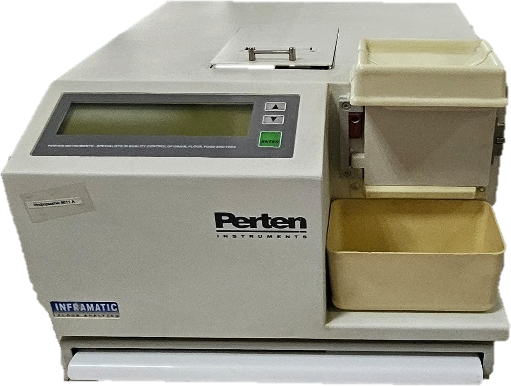
\includegraphics[width=\textwidth]{media/pish2/image18}
    \caption*{Рис. 1 - Анализатор «Инфраматик 8611»}
  \end{subfigure}%
  ~%
  \begin{subfigure}[b]{0.45\textwidth}
    
\includegraphics[width=\textwidth]{media/pish2/image19}
    \caption*{Рис. 2 - Спектрофотометр UV-1900i (Shimadzu, Япония)}
  \end{subfigure}
\end{figure}

\begin{multicols}{2}
Определение витаминного содержания проводилось при помощи
спектрофотометра UV-1900i (рисунок 2).

{\bfseries Результаты и обсуждение.} При разработке рецептуры безглютеновых
снэков с добавлением плодово-ягодных порошков ключевую роль играет
подбор образцов ягод и фруктов. При выборе образцов акцент был сделан на
то, что юго-восток Казахстана является родиной яблоки, север Казахстана
является территорией, где свободно растет облепиха, клюква, черная
смородина, черника и шиповник, на рынке Казахстана банан является одним
из самых распространенных и сравнительно дешевых фруктов. Исходя из
этого данные продукты являются легкодоступными.

Были проведены исследования качественных характеристик анализируемых
образцов на 100 г продукта.

Результаты анализа образцов на физико-химические показатели (содержание
белков, жиров, углеводов и клетчатки) представлены в виде сравнительной
диаграммы (рисунок 3).
\end{multicols}

{\bfseries Рис. 3 - Физико-химические показатели 7 разных видов порошка}

\emph{Образец №1 - банановый порошок, №2 - клюквенный порошок, №3 -
облепиховый порошок, №4 - порошок черной смородины, №5 - порошок
черники, №6 - порошок шиповник, №7 - яблочный порошок}

Данные, представленные на рисунке 3, свидетельствуют о том, что по
содержанию белка и жиров все образцы примерно на одном уровне, но
наибольшее содержание белка наблюдается в банановом порошке - 4,30\%, а
наибольшее содержание жира наблюдается в клюквенном порошке - 8,0\%.
Банановый и клюквенный порошки также отличаются высоким содержанием
углеводов - 56,3\% и 56,30\% соответственно. Порошки шиповника и яблока
содержат наибольшее количество клетчатки - 78,9\% и 74,5\%.

Результаты выявленного содержания витаминов В1, С, А, РР в отобранных
образцах плодово-ягодных порошков представлены в виде сравнительной
диаграммы (рисунок 4).

{\bfseries Рис. 4 - Содержание витаминов в 7 разных видах порошка}

\begin{multicols}{2}
\emph{Образец №1 - банановый порошок, №2 - клюквенный порошок, №3 -
облепиховый порошок, №4 - порошок черной смородины, №5 - порошок
черники, №6 - порошок шиповник, №7 ---\/- яблочный порошок}

Данные, представленные на рисунке 4 свидетельствует о том, что по
содержанию витамина В\textsubscript{1} лидирующая позиция у банана, с
показателем 12 \%, тогда как у шиповника она не превышает 0,8 \%.
Шиповник по содержанию витаминов С и А в несколько раз опережает другие
ягоды и фрукты с показателями 87,1 и 76,9 \%, уступая облепихе и черной
смородине, в это же время другие образцы показывают от 0,5 \% (черника).
По содержанию витамина РР лидирующую позицию держит банан (13 \%), во
всех остальных образцах они были в пределах 2,4-7,1 \%, что тоже
считается хорощим показателем.

На основе проведённого анализа качественных характеристик
плодово-ягодных порошков для обогащения безглютеновых снеков витаминами
и питательными веществами в качестве наиболее оптимальных вариантов были
выбраны следующие порошки: шиповниковый (образец №6), банановый (образец
№1), клюквенный (образец №2) и яблочный (образец №7).

Выбор шиповникового порошка обусловлен его лидирующими показателями по
содержанию витаминов C и A, а также высоким уровнем клетчатки, что
способствует укреплению иммунитета и улучшению пищеварения. Банановый
порошок был выбран за его высокое содержание белков, углеводов и
витаминов B1 и PP, что делает его отличным компонентом для повышения
энергетической ценности продукта. Клюквенный порошок демонстрирует
сбалансированный профиль питательных веществ, включая высокое содержание
углеводов и витамина C. Яблочный порошок выделяется значительным
количеством клетчатки, что делает его незаменимым для улучшения
функциональных характеристик снеков.

Таким образом, комбинация данных порошков обеспечивает оптимальное
сочетание вкусовых и питательных характеристик, а также удовлетворяет
требования к функциональному питанию.

{\bfseries Выводы.} Проведенное исследование качественных характеристик
плодово-ягодных порошков показало, что проанализированные образцы
бананового, клюквенного, облепихового, смородинного, черничного,
яблочного порошка и порошка шиповника могут эффективно использоваться
для обогащения витаминами безглютеновых снеков. В результате
сравнительного анализа было установлено, что различные виды порошков
имеют различные уровни содержания питательных веществ и витаминов, что
позволяет на основе этих данных выбрать оптимальные компоненты для
улучшения питательной ценности и функциональных свойств безглютеновых
снеков.

Для дальнейшей разработки рецептуры витаминизованного безглютенового
снэка из 7 порошков были выбраны 4, а именно порошки шиповника, банана,
клюквы и яблока, благодаря их высоким показателям витаминов, клетчатки и
углеводов. Использование вышеперечисленных порошков в качестве добавок в
производстве безглютеновых снеков может существенно улучшить рацион
питания людей с глютеновой непереносимостью, а также всех, кто
заинтересован в здоровом питании.

Таким образом, использование плодово-ягодных порошков в безглютеновых
снэках представляет собой эффективный способ обогащения рациона важными
питательными веществами и биоактивными соединениями. Это подчеркивает
необходимость дальнейших исследований и разработок в этой области для
повышения качества функциональных продуктов питания.

\emph{{\bfseries Финансирование.} Данное исследование финансировалось
Министерством сельского хозяйства Республики Казахстан в рамках
Научно-технической программы BR22886613 «Разработка инновационных
технологий по переработке и хранению сельскохозяйственной
растениеводческой продукции и сырья» на 2024-2026 годы по бюджетной
программе 267 «Повышение доступности знаний и научных исследований» по
подпрограмме 101 «Программно-целевое финансирование научных исследований
и мероприятий» по проекту «Разработка рецептуры витаминизованных
безглютеновых экструдированных снэков с добавлением плодово-ягодных
порошков».}
\end{multicols}

\begin{center}
{\bfseries Литература}
\end{center}

\begin{references}
1. Cleary L., Brennan C. The influence of a (1→3)(1→4)‐β‐d‐glucan rich
fraction from barley on the physico‐chemical properties and in vitro
reducing sugars release of durum wheat pasta // International Journal of
Food Science \& Technology.-2006.-Vol.41(8).- P.. 910--918.
DOI \\10.1111/j.1365-2621.2005.01141.x.

2. Padalino L., Mastromatteo M., Lecce L., Cozzolino F., Del Nobile M.
A. Optimization and \\characterization of gluten-free spaghetti enriched
with chickpea flour // International Journal of Food Sciences and
Nutrition. - 2015.- Vol.66(2).- P.148-158.
DOI 10.3109/09637486.2014.959897.

3. Барсукова Н. В., Решетников Д. А., Красильников В. Н. Пищевая
инженерия: технологии безглютеновых мучных изделий//Научный журнал НИУ
ИТМО. Серия «Процессы и аппараты пищевых производств». -2011. - № 1.-
C.9-17.

4. Рославцева Е. А., Сабельникова Е. А. Современные представления о
формах непереносимости глютена // Российский педиатрический журнал.-
2013.-№ 1.- С.21-27

5. Knai C., Pomerleau J., Lock K., McKee M. Getting children to eat more
fruit and vegetables: a systematic review // Preventive Medicine.-2006.-
Vol.42.-С.85--95. DOI 10.1016/j.ypmed.2005.11.012.

6. Maynard M., Gunnell D., Emmett P., Frankel S., Davey Smith G. Fruit,
vegetables and antioxidants in childhood and risk of adult cancer: The
Boyd Orr cohort // Journal of Epidemiology \& Community Health.- 2003.-
Vol. 57.- P. 218-225. DOI 10.1136/jech.57.3.218.

7. Antova T., Pattenden S., Nikiforov B., Leonardi G. S., Boeva B.,
Fletcher T. Nutrition and respiratory health in children in six Central
and Eastern European countries // Thorax.- 2003.-Vol. 58. -С. 231--236.
DOI 10.1136/thorax.58.3.231.

8. Christian P., Evans C. 14 Infancy, childhood, and adolescence //Human
Nutrition. - 2023. -P. 315. DOI 10.1093/hesc/9780198866657.003.0018

9. Hampl J. S., Betts N. M., Benes B. A. The ``Age +5'' rule; comparisons
of dietary fiber intake among 4--10 year old children // Journal of the
American Dietetic Association.- 1998.- Vol. 98.- P. 1418-1423. DOI
10.1016/S0002-8223(98)00320-4.

10. Ames B. M., Shigena M. K., Hagen T. M. Oxidants, antioxidants and the
degenerative diseases of aging // Proceedings of the National Academy of
Science U.S.A.- 1993.- Vol. 90.- P. 7915-7922. DOI
10.1073/pnas.90.17.7915.

11. Mintel. How Snack Brands Can Win the Generation Game. Industry Trend
Insight. -- Mintel,
2024. \href{https://store.mintel.com/report/how-snack-brands-can-win-the-generation-game}{https://store.mintel.com}.
Date of address: 05.01.2025)
\end{references}

\begin{center}
{\bfseries References}
\end{center}

\begin{references}
1. Cleary L., Brennan C. The influence of a (1→3)(1→4)‐β‐d‐glucan rich
fraction from barley on the physico‐chemical properties and in vitro
reducing sugars release of durum wheat pasta // International Journal of
Food Science \& Technology.-2006.-Vol.41(8).- P.. 910--918.
DOI \\10.1111/j.1365-2621.2005.01141.x.

2. Padalino L., Mastromatteo M., Lecce L., Cozzolino F., Del Nobile M.
A. Optimization and \\characterization of gluten-free spaghetti enriched
with chickpea flour // International Journal of Food Sciences and
Nutrition. - 2015.- Vol.66(2).- P.148-158.
DOI 10.3109/09637486.2014.959897.

3. Barsukova N. V., Reshetnikov D. A., Krasil' nikov V. N.
Pishhevaja inzhenerija: tehnologii \\bezgljutenovyh muchnyh
izdelij//Nauchnyj zhurnal NIU ITMO. Serija «Processy i apparaty
pishhevyh proizvodstv». -2011. - № 1.- C.9-17.{[}in Russian{]}

4. Roslavceva E. A., Sabel' nikova E. A. Sovremennye
predstavlenija o formah neperenosimosti gljutena // Rossijskij
pediatricheskij zhurnal.- 2013.-№ 1.- S.21-27.{[}in Russian{]}

5. Knai C., Pomerleau J., Lock K., McKee M. Getting children to eat more
fruit and vegetables: a systematic review // Preventive Medicine.-2006.-
Vol.42.-С.85--95. DOI 10.1016/j.ypmed.2005.11.012.

6. Maynard M., Gunnell D., Emmett P., Frankel S., Davey Smith G. Fruit,
vegetables and antioxidants in childhood and risk of adult cancer: The
Boyd Orr cohort // Journal of Epidemiology \& Community Health.- 2003.-
Vol. 57.- P. 218-225. DOI 10.1136/jech.57.3.218.

7. Antova T., Pattenden S., Nikiforov B., Leonardi G. S., Boeva B.,
Fletcher T. Nutrition and respiratory health in children in six Central
and Eastern European countries // Thorax.- 2003.-Vol. 58. -С. 231--236.
DOI 10.1136/thorax.58.3.231.

8. Christian P., Evans C. 14 Infancy, childhood, and adolescence //Human
Nutrition. - 2023. -P. 315. DOI 10.1093/hesc/9780198866657.003.0018

9. Hampl J. S., Betts N. M., Benes B. A. The ``Age +5'' rule; comparisons
of dietary fiber intake among 4--10 year old children // Journal of the
American Dietetic Association.- 1998.- Vol. 98.- P. 1418-1423. DOI
10.1016/S0002-8223(98)00320-4.

10. Ames B. M., Shigena M. K., Hagen T. M. Oxidants, antioxidants and the
degenerative diseases of aging // Proceedings of the National Academy of
Science U.S.A.- 1993.- Vol. 90.- P. 7915-7922. DOI
10.1073/pnas.90.17.7915.

11. Mintel. How Snack Brands Can Win the Generation Game. Industry Trend
Insight. -- Mintel,
2024. \href{https://store.mintel.com/report/how-snack-brands-can-win-the-generation-game}{https://store.mintel.com}.
Date of address: 05.01.2025)
\end{references}

\begin{authorinfo}
\emph{{\bfseries Сведения об авторах}}

Қабылда А.И. - кандидат сельскохозяйственных наук, ведущий научный
сотрудник, АФ ТОО «Казахский научно - исследовательский институт
перерабатывающей и пищевой промышленности», Астана, Казахстан, е-mail:\\
\href{mailto:anara121579@gmail.com}{\nolinkurl{anara121579@gmail.com}};

Жармаханова А.С. - магистр естественных наук, младший научный сотрудник,
АФ ТОО «Казахский научно - исследовательский институт перерабатывающей и
пищевой промышленности», Астана, Казахстан, e-mail:\\
\href{mailto:arukydyrkozha77@gmail.com}{\nolinkurl{arukydyrkozha77@gmail.com}};

Кожухова Ж.С. - магистрант, младший научный сотрудник, АФ ТОО «Казахский
научно-исследовательский институт перерабатывающей и пищевой
промышленности», Астана, Казахстан, е-mail:
\href{mailto:jansa1612@gmail.com}{\nolinkurl{jansa1612@gmail.com}}

\emph{{\bfseries Information about the authors}}

Kabylda A. I. -- Candidate of Agricultural Sciences, Senior Researcher,
Astana branch of LLP "Kazakh Research Institute of Processing and Food
Industry", Astana, Kazakhstan, е-mail:
\href{mailto:anara121579@gmail.com}{\nolinkurl{anara121579@gmail.com}};

Zharmakhanova A. S. -- Master of Natural Sciences, Junior Researcher,
Astana branch of LLP "Kazakh Research Institute of Processing and Food
Industry", Astana, Kazakhstan, e-mail: arukydyrkozha77@gmail ;

Kozhukhova Z. S. -- Master' s Student, Junior Researcher,
Astana branch of LLP "Kazakh Research Institute of Processing and Food
Industry", Astana, Kazakhstan, е-mail:
\href{mailto:jansa1612@gmail.com}{\nolinkurl{jansa1612@gmail.com}},
\end{authorinfo}
